\documentclass[11pt]{article}

\usepackage[utf8]{inputenc}
\usepackage[T1]{fontenc}
\usepackage[margin=1in]{geometry}
\usepackage{graphicx}
\usepackage{amsmath}
\usepackage{booktabs}
\usepackage{array}
\usepackage{longtable}
\usepackage{adjustbox}
\usepackage{caption}
\usepackage{subcaption}
\usepackage{authblk}
\usepackage{hyperref}
\usepackage{cite}
\usepackage{setspace}
\onehalfspacing

\hypersetup{
  colorlinks=true,
  linkcolor=blue,
  citecolor=blue,
  urlcolor=blue
}

\title{\textbf{Strong Within-Domain EEG Workload Decoding Fails to Transport
Across Heterogeneous Task and Device Domains: A Prospectively Evaluated
Negative Methods Study}}

\author[1]{Arush Ravipati$^{\ast}$}
\author[1]{Abhijay Gangarapu$^{\ast}$}
\affil[1]{Independent Researcher}

\date{June 2026}

\begin{document}

\maketitle
\begingroup
\renewcommand{\thefootnote}{}
\footnotetext{$^{\ast}$These authors contributed equally to this work.}
\endgroup

\begin{abstract}
EEG cognitive-workload classifiers frequently achieve high accuracy
\textit{within} a single dataset, yet within-dataset performance is not
evidence that a decoder \textit{transports} to a new device, task, or cohort.
We separate these two questions with a sequential, preregistration-style design
across three provenance-distinct datasets: PhysioNet EEG During Mental
Arithmetic Tasks (MAT; development), STEW (an exploratory, non-comparable
cross-task/cross-device sensitivity dataset), and COG-BCI (Hinss et al.\ 2023;
a single untouched prospective test). Within each development dataset,
subject-baseline mean-subtraction calibration decoded workload above chance at
the subject level: macro subject-level ROC-AUC was $0.880102$ within MAT
(full-pipeline within-subject label-permutation $p = 0.004975$, 200
permutations) and $0.839498$ within STEW ($p = 0.004975$). Mean subtraction was
not proven superior to absolute features in either dataset (paired confidence
intervals crossed zero). When the frozen, unit-compatible pipeline was applied
across datasets, the predeclared MAT$\rightarrow$STEW mean-subtraction
\textit{transport failed} (macro subject AUC $0.447598$, below chance, not
better than absolute $0.472045$). A post-hoc z-scoring observation on the same
transport (AUC $0.682823$) was the only above-chance mode; we treated it strictly
as a hypothesis to be tested, froze the entire pipeline, and evaluated it
\textit{exactly once} on untouched COG-BCI. That prospective test also failed:
all three calibration modes transported below chance (z-scoring $0.435961$, mean
subtraction $0.392153$, absolute $0.367875$; $n = 29$), and the primary paired
contrast (z-scoring $-$ mean subtraction) had mean $\Delta = +0.043807$ with a
$95\%$ CI $[-0.076359, +0.175233]$ that includes zero. Under the specific
task/device/reference shifts tested here, baseline-relative preprocessing
supported within-dataset workload discrimination but did \textit{not} provide
supported transportability of a MAT-trained workload decoder. We report this as
a rigorous negative transport/reproducibility result.
\end{abstract}

\section{Introduction}

Cognitive workload modulates theta- and alpha-band EEG activity during
arithmetic, working-memory, and attention tasks
\cite{klimesch1999, gevins1997, zyma2019}. These signatures motivate EEG-based
passive brain--computer interfaces and workload monitors, but they do not by
themselves establish \textit{generalizable} prediction. Scalp EEG features also
encode stable differences between participants, reference montages, electrode
layouts, amplifier hardware, task timing, and recording systems. A model can
therefore score well by exploiting subject- or dataset-specific structure
rather than a task-general workload signal \cite{lotte2018, jayaram2016}. The
central methodological problem we address is the gap between within-dataset
decoding and cross-domain transport: leave-one-subject-out (LOSO) accuracy
inside one dataset is routinely high, yet that number is not a measurement of
whether the same decoder works on a different device and task
\cite{zanini2018, congedo2017}.

Subject-relative calibration is a natural candidate for closing that gap.
Expressing each subject's task windows relative to that subject's own resting
baseline --- by subtracting the baseline mean (mean subtraction) or by
standardizing to baseline mean and standard deviation (z-scoring) --- is a
plausible route to features that are less sensitive to per-subject and
per-device offsets and scales \cite{vidaurre2011}. We emphasize at the outset
that baseline-relative calibration is introduced here only as a candidate
calibration step, \textbf{not} as a proven mechanism and \textbf{not} as a
claim about neural generators.

This manuscript asks one question: does subtracting or standardizing each
subject's resting EEG baseline produce a workload-decoding signal that
\textit{transfers} across provenance-distinct EEG datasets (different devices
and tasks), or only \textit{within} each dataset? We answer it with a
deliberately sequential, hypothesis-controlled design. Two datasets (MAT and
STEW) are used only for development; a third dataset (COG-BCI) is held
completely untouched and used for a single, checksum-locked prospective test of
the one hypothesis that the development phase generated. We report every
decisive outcome exactly as executed, including the failures, and constrain all
claims to analyses that were actually run in the repository. We do not report
coupling analyses, source reconstruction, anatomical-generator claims, or any
graded cross-dataset confirmation, because those analyses are not part of the
verified evidence behind this paper.

\section{Materials and Methods}

\subsection{Sequential hypothesis-control design}

The study has three stages with fixed, non-interchangeable roles
(Figure~\ref{fig:flow}). \textbf{Development:} MAT and STEW are used to develop
and stress-test the candidate calibration method and to generate hypotheses.
\textbf{Post-hoc hypothesis:} an observation made \textit{after} viewing the
MAT$\rightarrow$STEW transport is allowed to generate a single new hypothesis,
which is then frozen. \textbf{Prospective test:} COG-BCI is an untouched
dataset reserved for exactly one evaluation of the frozen hypothesis. MAT and
STEW count only as development evidence and may not serve as prospective
validation; COG-BCI is never inspected or modeled until its frozen protocol and
a provenance audit have passed.

\subsection{Datasets and raw-data provenance}

Dataset roles, devices, sampling rates, baselines, and subject counts are
summarized in Table~\ref{tab:datasets}.

\textbf{MAT (development).} The PhysioNet EEG During Mental Arithmetic Tasks
dataset \cite{physionet_eegmat, zyma2019, goldberger2000} was audited from the
official raw EDF files: 36 subjects, 72 EDF files, 500\,Hz, microvolt units, a
standard 10--20 montage. Files ending in \texttt{\_1} are rest/background and
files ending in \texttt{\_2} are mental arithmetic. A corrected balanced
protocol was used with equal scored-rest and scored-task window counts per
subject and no overlap between calibration and scored segments.

\textbf{STEW (exploratory sensitivity).} The STEW dataset
\cite{stew_dataset} comprises 48 subjects recorded at 128\,Hz with a 14-channel
Emotiv EPOC+ headset under low- versus high-workload multitasking conditions.
STEW is explicitly treated as a \textbf{non-comparable} cross-task/cross-device
sensitivity dataset, \textbf{not} a strict replication: it differs from MAT in
task, device, montage, reference, sampling rate, and amplitude units. The
official IEEE DataPort STEW source was used; per-subject calibration, scored
rest, and scored task were drawn from disjoint segments (14/14/14 windows per
subject).

\textbf{COG-BCI (untouched prospective test).} The COG-BCI database
\cite{hinss2023} provides multi-session EEG including a Multi-Attribute Task
Battery (MATB) and resting-state recordings on a BrainProducts system. A
source provenance audit confirmed 29 readable subjects, the eight required
channels, 500\,Hz sampling, and the presence of eyes-open rest and
MATB-difficult conditions. The primary paradigm was predeclared as MATB
(highest level $=$ MATB difficult), chosen by construct match to MAT arithmetic
\textbf{before} any outcome was seen; N-back, eyes-closed rest, other MATB
levels, and sessions S2/S3 were prespecified out of scope and were never
analyzed.

\subsection{Frozen feature space and unit-incompatibility audit}

Within-dataset analyses used a frozen no-gamma 184-feature, 8-channel family.
Gamma bands were removed. Cross-dataset transport, however, faces a unit
problem: MAT amplitudes are in microvolts, whereas STEW values are undocumented
raw 16-bit Emotiv counts for which no verified microvolt conversion exists
(archive, IEEE page, and publication were all checked). We therefore restricted
all transport analyses to the \textbf{96 features proven invariant under the
positive affine transform $x \rightarrow a\,x + b$ ($a > 0$)}: skewness,
kurtosis, Hjorth mobility, Hjorth complexity, spectral entropy, relative
bandpower in $\delta$, $\theta$, $\alpha$, $\beta$, and the $\theta/\alpha$,
$\beta/\alpha$, $\theta/\beta$ ratios, across the 8 channels. Amplitude,
variance, absolute power, Hjorth activity, and Shannon entropy were excluded
because they are not scale/offset invariant. The eight harmonized channels were
F3, F4, F7, F8, O1, O2, T7$\rightarrow$T3, and T8$\rightarrow$T4.

\subsection{Sampling representation (transparent amendment)}

The transport-compatible feature set is scale- and offset-invariant but is
\textbf{not} sampling-rate-invariant. Because the development transport pipeline
(MAT$\rightarrow$STEW) trained the source model at 128\,Hz, both the source
(MAT) and the target (COG-BCI) must be represented at the same rate. An earlier
draft of the COG-BCI protocol stated ``500\,Hz native --- no resample,'' which
conflicted with the frozen 128\,Hz transport representation. This was corrected
\textbf{before any COG-BCI predictive metric was computed} and purely for
representational consistency: both MAT and COG-BCI are resampled from 500\,Hz to
128\,Hz with \texttt{scipy.signal.resample\_poly} (\texttt{up=32},
\texttt{down=125}) before the frozen 96 features are extracted. Native-500-Hz
COG-BCI analysis was forbidden from the primary verdict. This amendment changed
only the sampling representation, not the model, features, channels, endpoint,
or comparator.

\subsection{Calibration modes}

Three feature representations were compared throughout: (1) absolute features;
(2) mean subtraction relative to the subject's resting baseline (the
development-selected candidate); and (3) z-scoring relative to the subject's
resting baseline (a predeclared secondary diagnostic). In every transport
analysis, per-subject calibration statistics were computed from the subject's
\textbf{unlabeled} resting-baseline segment only, disjoint from the scored
segments.

\subsection{Model, evaluation, and leakage controls}

The fixed model was L2-regularized logistic regression
($C = 1.0$, \texttt{solver = liblinear}, \texttt{class\_weight = balanced},
\texttt{max\_iter = 5000}) \cite{sklearn}; no label-dependent hyperparameter
search was performed. The primary unit of inference was macro subject-level
ROC-AUC. Within-dataset analyses used strict LOSO: in each fold the held-out
subject contributed nothing to calibration statistics, imputation, scaling, or
model fitting. Transport analyses fit the imputer, scaler, and model on the
\textbf{source dataset only} and used target labels solely to score, never to
fit, select, preprocess, or tune. Uncertainty was quantified by subject-level
bootstrap confidence intervals, and within-dataset significance by full-pipeline
within-subject label-permutation nulls (200 permutations, full LOSO refit per
permutation). EEG I/O used MNE-Python \cite{mne, gramfort2013}.

\subsection{COG-BCI untouched one-shot prospective protocol}

The COG-BCI test was frozen, checksum-locked, input-hash-verified, and executed
exactly once. The frozen configuration trained on MAT only (rest versus
arithmetic). The target was COG-BCI \texttt{ses-S1}: the unlabeled
calibration baseline was the first 30\,s of \texttt{RS\_Beg\_EO} (eyes-open
rest); scored rest was the first 30\,s of \texttt{RS\_End\_EO} (label 0); scored
workload was the first 30\,s of \texttt{MATBdiff} (label 1). Windows were 4\,s
with 50\% overlap, yielding 14 rest and 14 task windows per subject; all 29
subjects were scored with no pre-outcome exclusion. The primary endpoint was the
macro subject-level ROC-AUC of z-scoring; the primary comparison was the paired
subject-bootstrap $\Delta$AUC of z-scoring minus mean subtraction. The locked
classification rule was: \emph{full success} requires z-scoring above chance and
a primary CI excluding zero positively; \emph{partial} requires z-scoring above
chance with the CI including zero; \emph{failure} otherwise (z-scoring at/below
chance, or not outperforming mean subtraction). No retuning, task switching,
channel expansion, feature reselection, or endpoint change was permitted after
outcomes were accessed.

\subsection{Run-once controls and reproducibility}

The frozen run materials (configuration YAML and execution script) were
SHA-256-checksummed before execution; the run-time record and the live committed
files were verified byte-identical. A single run marker
(\texttt{RUN\_MARKER.json}) records one execution, and the script aborts if any
result output already exists, preventing a second result-producing run. All 29
locked input files were SHA-256-recorded in an input-hash manifest. An
independent read-only integrity audit confirmed exactly one execution, internal
consistency of all reported values across JSON/CSV/Markdown, alignment of
checksums, and that the failure classification follows the predeclared rule.

\section{Results}

\subsection{Provenance and pipeline validity}

Raw MAT EDFs were integrity-verified (72/72 SHA-256 matched the validated MAT
provenance manifest). The STEW measurement-unit ambiguity was resolved
conservatively by restricting transport to the 96 positive-affine-invariant
features, frozen before any transfer result was viewed. For COG-BCI, the source
provenance audit passed (29/29 subjects readable, 8 locked channels, eyes-open
rest and MATB-difficult present), the frozen config/script checksums matched the
run-time and committed files exactly, and the one-shot script ran cleanly to
completion. The leakage-free design (source-only fitting; unlabeled-baseline
calibration; disjoint calibration and scored segments) was verified.

\subsection{Within-MAT workload decoding is above chance}

Within MAT, mean-subtraction calibration decoded rest versus mental arithmetic
above chance at the subject level: macro subject-level ROC-AUC $= 0.880102$
(Table~\ref{tab:within}, Figure~\ref{fig:within}). The full-pipeline
within-subject label-permutation null had mean $0.500600$, $95\%$ interval
$[0.441057, 0.553729]$, and empirical $p = 0.004975$ (200 permutations).
Mean subtraction was \textbf{not} proven superior to absolute features
($0.841553$): the paired mean-subtraction $-$ absolute $95\%$ CI
$[-0.018566, +0.093112]$ includes zero. This is a within-dataset result only.

\subsection{Within-STEW exploratory sensitivity}

Within STEW, mean-subtraction calibration decoded low versus high workload above
chance at the subject level: macro subject-level ROC-AUC $= 0.839498$
(permutation null mean $0.502071$, $95\%$ $[0.458830, 0.539908]$,
$p = 0.004975$). As in MAT, mean subtraction was not proven superior to absolute
features ($0.815795$; paired CI $[-0.013180, +0.060717]$ includes zero).
z-scoring was numerically highest within STEW ($0.898703$) but is a secondary
diagnostic only; per the frozen protocol the candidate method was not switched
because STEW favored z-scoring. STEW remains exploratory, cross-task,
cross-device, and non-comparable --- supportive sensitivity evidence
\textit{inside} STEW, not replication or confirmation.

\subsection{MAT$\rightarrow$STEW mean-subtraction transport fails}

This is the central negative pivot. Under the frozen, unit-invariant transport
pipeline (train on MAT only, test on STEW), the predeclared candidate (mean
subtraction) \textbf{failed to transport}: macro subject AUC $= 0.447598$,
\textit{below chance}, and not better than absolute ($0.472045$; paired CI
$[-0.070057, +0.022646]$ includes zero) (Table~\ref{tab:transport},
Figure~\ref{fig:transport}). Strong within-dataset decoding (0.84--0.88) did not
carry over to a different device and task.

\subsection{Post-hoc z-scoring observation (hypothesis-generating only)}

Of the three modes, only z-scoring transported above chance on
MAT$\rightarrow$STEW (macro subject AUC $= 0.682823$). Although the z-scoring
computation was predeclared and verified leakage-free, its
\textit{elevation as a method of interest} occurred only \textit{after} viewing
the transport results, so it is post-hoc. We therefore treated it strictly as
\textbf{hypothesis-generating}, not as confirmatory evidence: a single new
hypothesis --- that under severe cross-device/task scale shift, subject-level
standardization might transport better than centering --- to be frozen and
tested once on an untouched dataset. We do not claim z-scoring transfers.

\subsection{Frozen one-shot COG-BCI prospective test fails below chance}

The frozen hypothesis was tested exactly once on untouched COG-BCI. All three
calibration modes transported \textit{below chance}: z-scoring $0.435961$
(subject-bootstrap $95\%$ CI $[0.359602, 0.509338]$), mean subtraction
$0.392153$, and absolute $0.367875$ ($n = 29$; Table~\ref{tab:cogbci},
Figure~\ref{fig:cogbci}). The primary paired contrast, z-scoring minus mean
subtraction, had mean $\Delta = +0.043807$ with a $95\%$ CI
$[-0.076359, +0.175233]$ that includes zero; the secondary contrast (z-scoring
minus absolute) was $+0.068086$, CI $[-0.060173, +0.190715]$, also including
zero. Under the locked rule, z-scoring is below chance, so the above-chance
precondition for success or partial success is not met, and the primary
superiority CI includes zero. The classification is \textbf{failure}: the
MAT$\rightarrow$STEW z-scoring elevation did not replicate.

\subsection{Final decision}

Combining the predeclared MAT$\rightarrow$STEW mean-subtraction transport failure
with the prospective COG-BCI failure of the post-hoc z-scoring hypothesis,
cross-device/cross-task \textbf{transfer} of the MAT-trained decoder is
\textbf{not supported} under the tested domain shifts, for any of absolute, mean
subtraction, or z-scoring calibration. The within-dataset MAT and STEW findings
are unchanged and remain within-dataset evidence only. The project verdict was
recorded as \texttt{PROSPECTIVE\_ZSCORE\_TRANSPORT\_FAILED\_WRITE\_NEGATIVE\_METHODS\_PAPER}.

\begin{table}[ht]
\centering
\caption{Datasets and their fixed roles in the sequential design.}
\label{tab:datasets}
\small
\adjustbox{max width=\textwidth}{%
\begin{tabular}{lllllr}
\toprule
Dataset & Role & Task / contrast & Baseline & Device / sampling & Subjects \\
\midrule
MAT & Development & Rest vs.\ mental arithmetic & Resting block & 10--20, $\mu$V, 500\,Hz & 36 \\
STEW & Exploratory sensitivity & Low vs.\ high workload & Low-load segment & Emotiv EPOC+ 14ch, counts, 128\,Hz & 48 \\
COG-BCI & Untouched prospective test & Eyes-open rest vs.\ MATB-difficult & Eyes-open rest & BrainProducts, $\mu$V, 500\,Hz$\rightarrow$128\,Hz & 29 \\
\bottomrule
\end{tabular}}
\par\vspace{2pt}
\footnotesize STEW units are undocumented raw 16-bit counts; cross-dataset
transport therefore used only the 96 scale/offset-invariant features. COG-BCI
was resampled to 128\,Hz to match the frozen transport representation.
\end{table}

\begin{table}[ht]
\centering
\caption{Within-domain subject-level decoding (L2 logistic regression, LOSO).
Mean subtraction is above chance within each dataset but not proven superior to
absolute features (paired CIs include zero). z-scoring within STEW is a
secondary diagnostic only.}
\label{tab:within}
\small
\begin{tabular}{lllr}
\toprule
Dataset & Calibration & Macro subject AUC & Permutation $p$ \\
\midrule
MAT  & absolute              & 0.841553 & --- \\
MAT  & mean subtraction      & \textbf{0.880102} & 0.004975 \\
MAT  & z-scoring (diagnostic)& 0.816327 & --- \\
STEW & absolute              & 0.815795 & --- \\
STEW & mean subtraction      & \textbf{0.839498} & 0.004975 \\
STEW & z-scoring (diagnostic)& 0.898703 & --- \\
\bottomrule
\end{tabular}
\par\vspace{2pt}
\footnotesize Paired mean-subtraction $-$ absolute $95\%$ CIs:
MAT $[-0.018566, +0.093112]$; STEW $[-0.013180, +0.060717]$ (both include zero).
\end{table}

\begin{table}[ht]
\centering
\caption{MAT$\rightarrow$STEW exploratory transport (train MAT, test STEW; 96
scale/offset-invariant features; 48 target subjects). The predeclared candidate
(mean subtraction) transports below chance; z-scoring is the only above-chance
mode and is post-hoc/hypothesis-generating only.}
\label{tab:transport}
\small
\begin{tabular}{lrl}
\toprule
Calibration & Macro subject AUC & Above chance? \\
\midrule
absolute               & 0.472045 & No \\
mean subtraction (candidate) & \textbf{0.447598} & No (below chance) \\
z-scoring (post-hoc diagnostic) & 0.682823 & Yes \\
\bottomrule
\end{tabular}
\par\vspace{2pt}
\footnotesize Paired mean-subtraction $-$ absolute $95\%$ CI
$[-0.070057, +0.022646]$ (includes zero).
\end{table}

\begin{table}[ht]
\centering
\caption{COG-BCI untouched one-shot prospective test (MAT$\rightarrow$COG-BCI;
29 target subjects). All three modes transport below chance; the primary paired
contrast includes zero. Classification: failure.}
\label{tab:cogbci}
\small
\adjustbox{max width=\textwidth}{%
\begin{tabular}{llrll}
\toprule
Method & Role & Macro subject AUC & Subject $95\%$ CI & Above chance? \\
\midrule
z-scoring        & primary            & 0.435961 & $[0.359602, 0.509338]$ & No \\
mean subtraction & primary comparator & 0.392153 & $[0.310697, 0.476258]$ & No \\
absolute         & secondary comparator & 0.367875 & $[0.286590, 0.456725]$ & No \\
\midrule
\multicolumn{5}{l}{Primary $\Delta$AUC (z-scoring $-$ mean subtraction): mean $+0.043807$, $95\%$ CI $[-0.076359, +0.175233]$ (includes zero).}\\
\multicolumn{5}{l}{Secondary $\Delta$AUC (z-scoring $-$ absolute): mean $+0.068086$, $95\%$ CI $[-0.060173, +0.190715]$ (includes zero).}\\
\bottomrule
\end{tabular}}
\end{table}

\begin{figure}[ht]
\centering
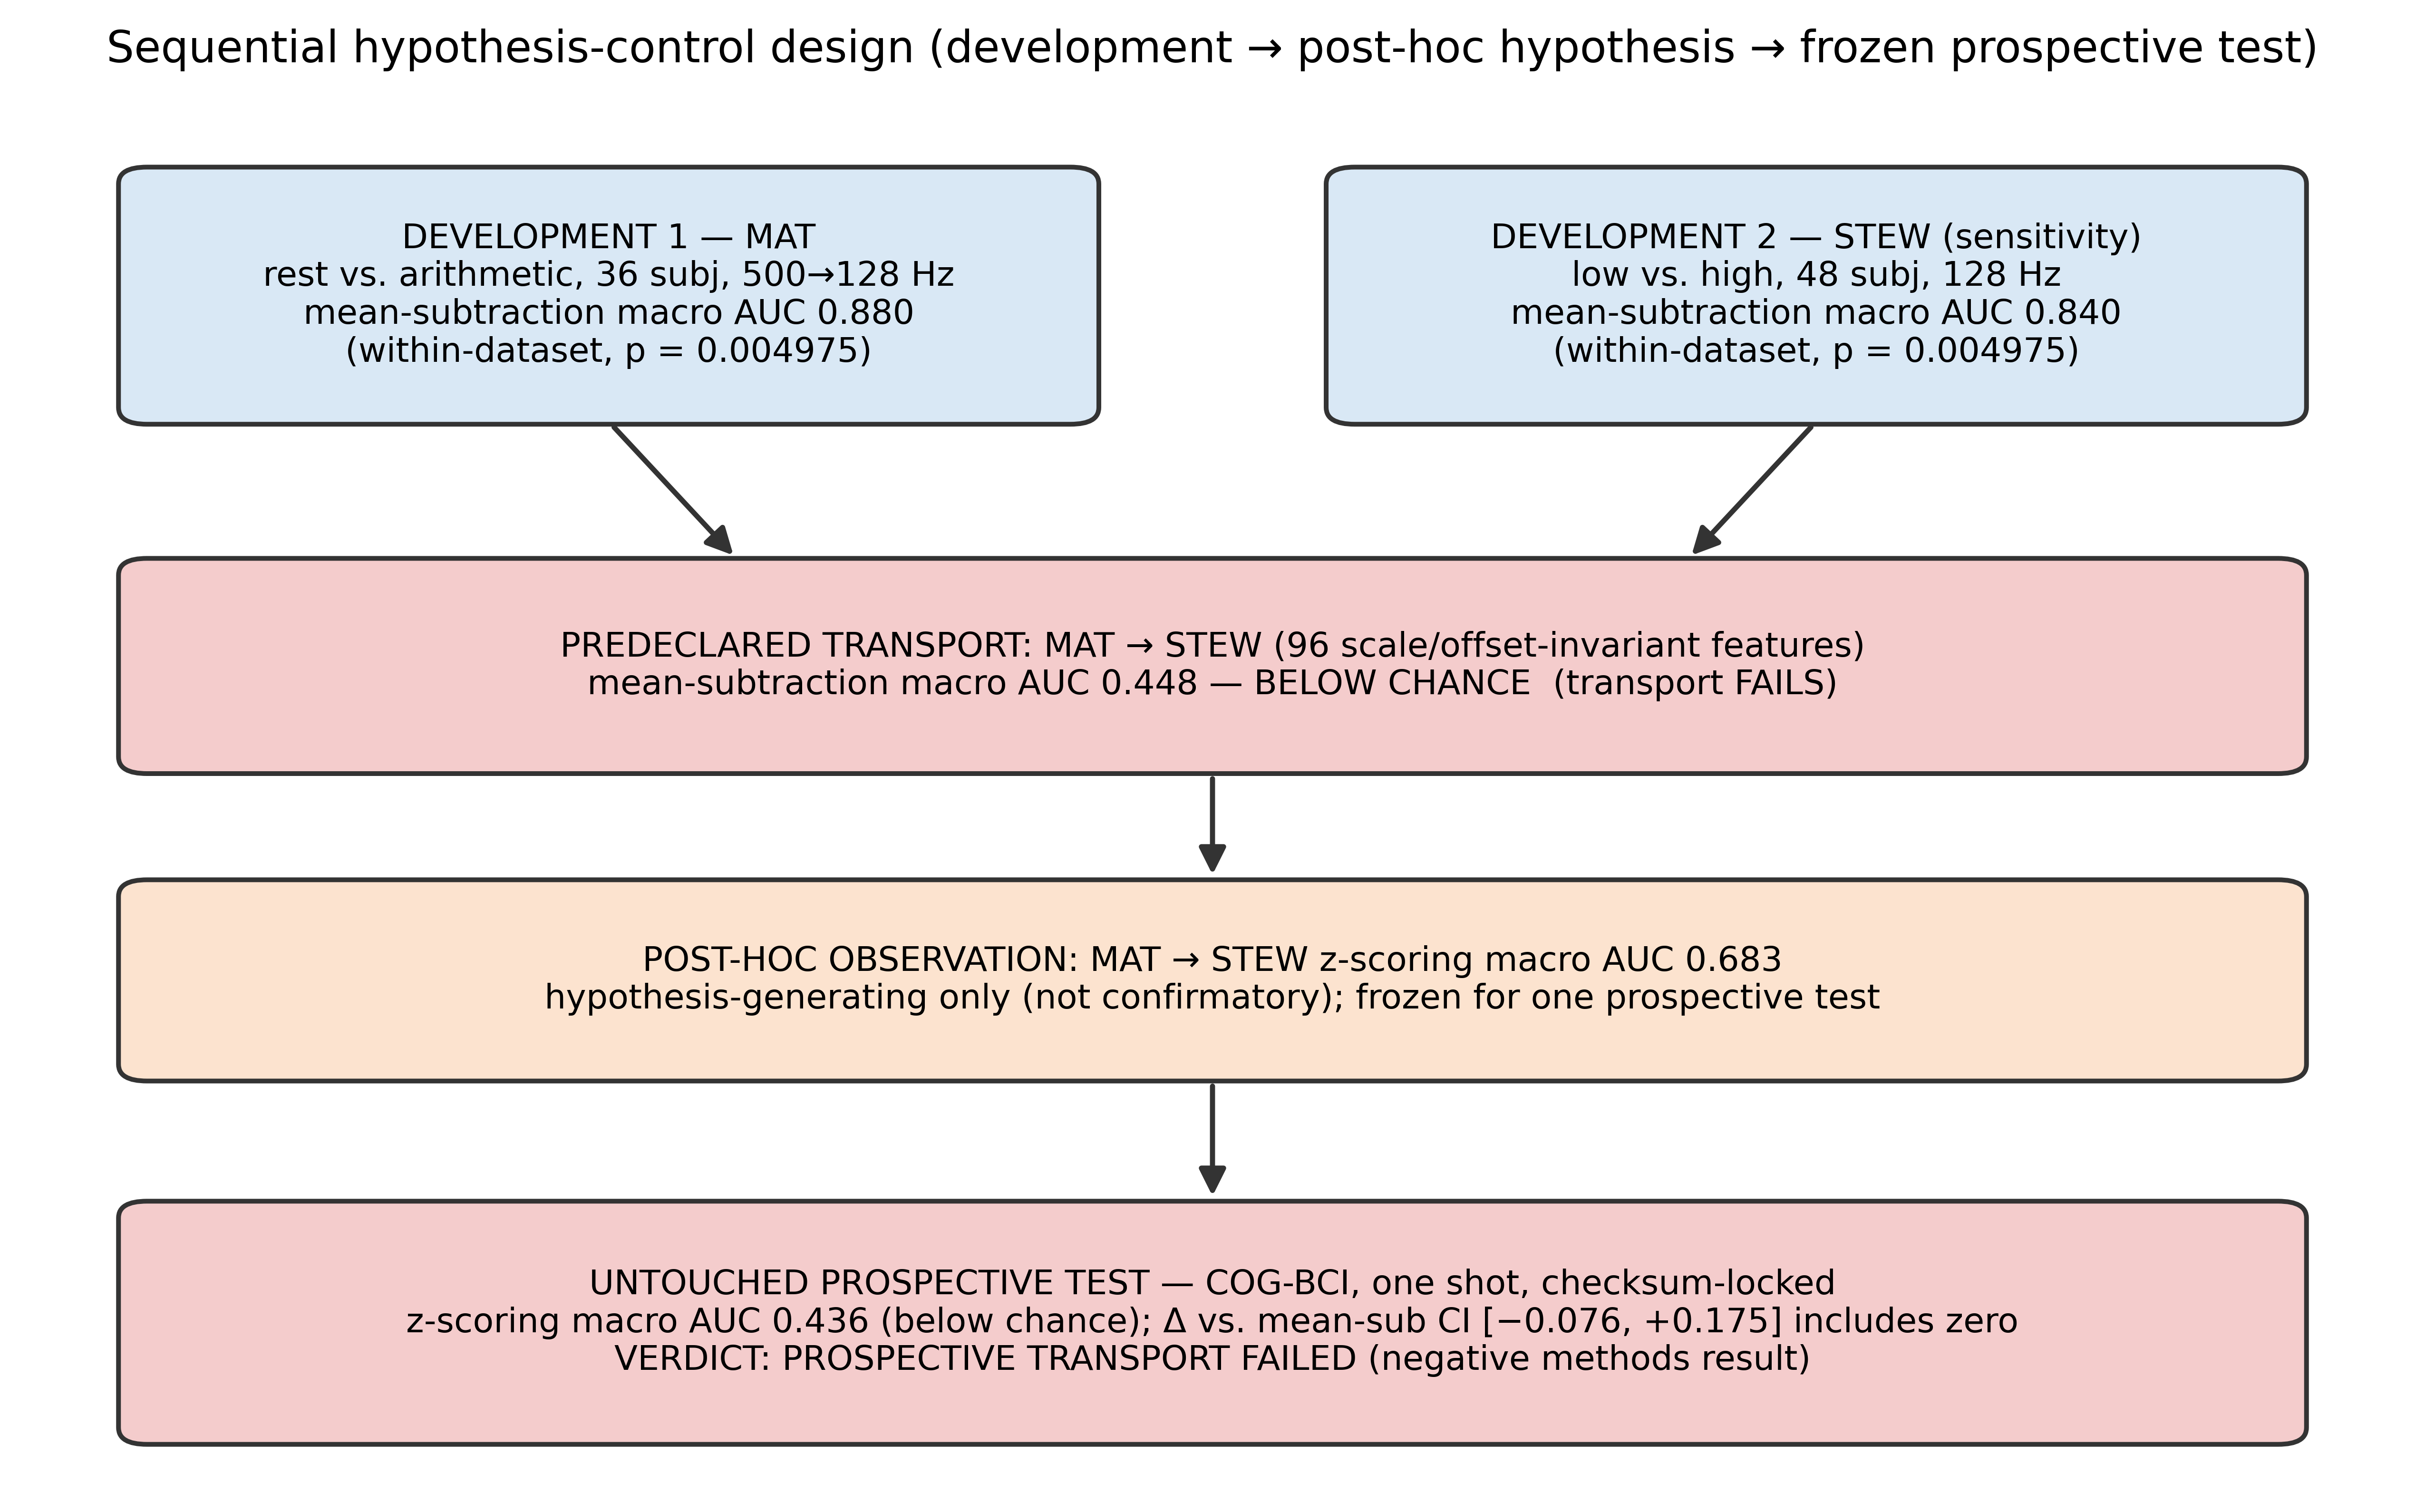
\includegraphics[width=0.95\linewidth]{../figures/figure_neg_design_flow.png}
\caption{Sequential hypothesis-control design. Two development datasets (MAT,
STEW) yield strong within-dataset decoding; the predeclared MAT$\rightarrow$STEW
mean-subtraction transport fails below chance; a post-hoc z-scoring observation
generates a single hypothesis that is frozen and tested exactly once on
untouched COG-BCI, where it also fails below chance.}
\label{fig:flow}
\end{figure}

\begin{figure}[ht]
\centering
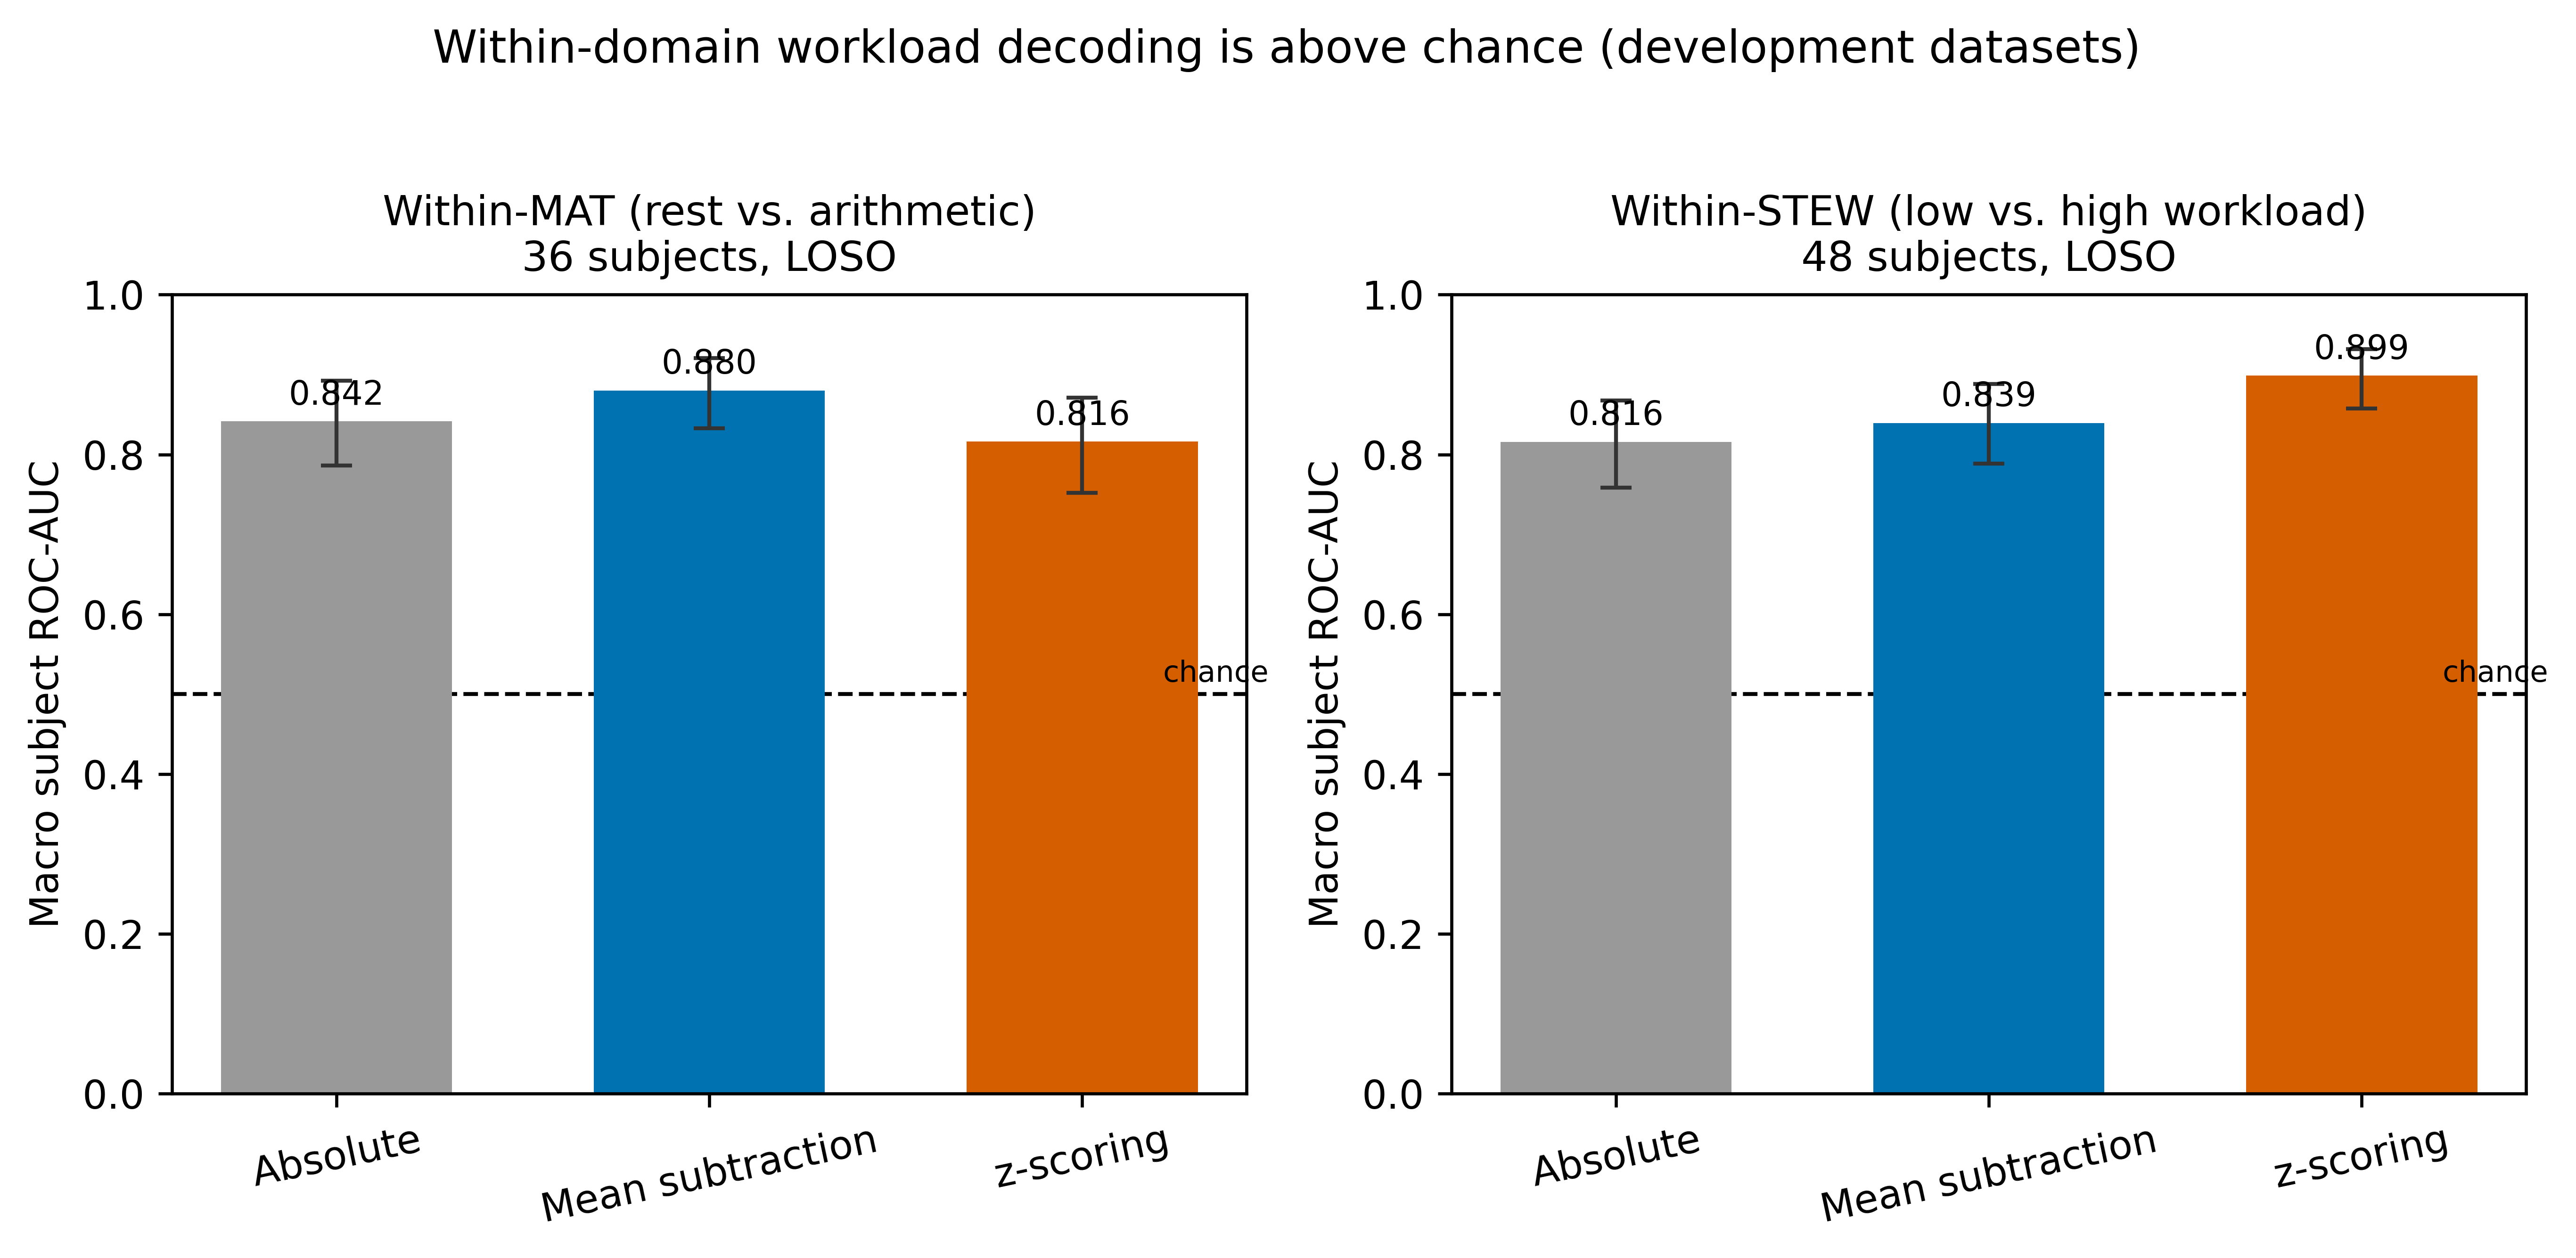
\includegraphics[width=0.92\linewidth]{../figures/figure_neg_within_domain_auc.png}
\caption{Within-domain macro subject-level ROC-AUC by calibration mode for MAT
(left) and STEW (right). Error bars are subject-bootstrap $95\%$ CIs; the dashed
line marks chance (0.5). Mean-subtraction permutation $p = 0.004975$ in both
datasets (200 permutations).}
\label{fig:within}
\end{figure}

\begin{figure}[ht]
\centering
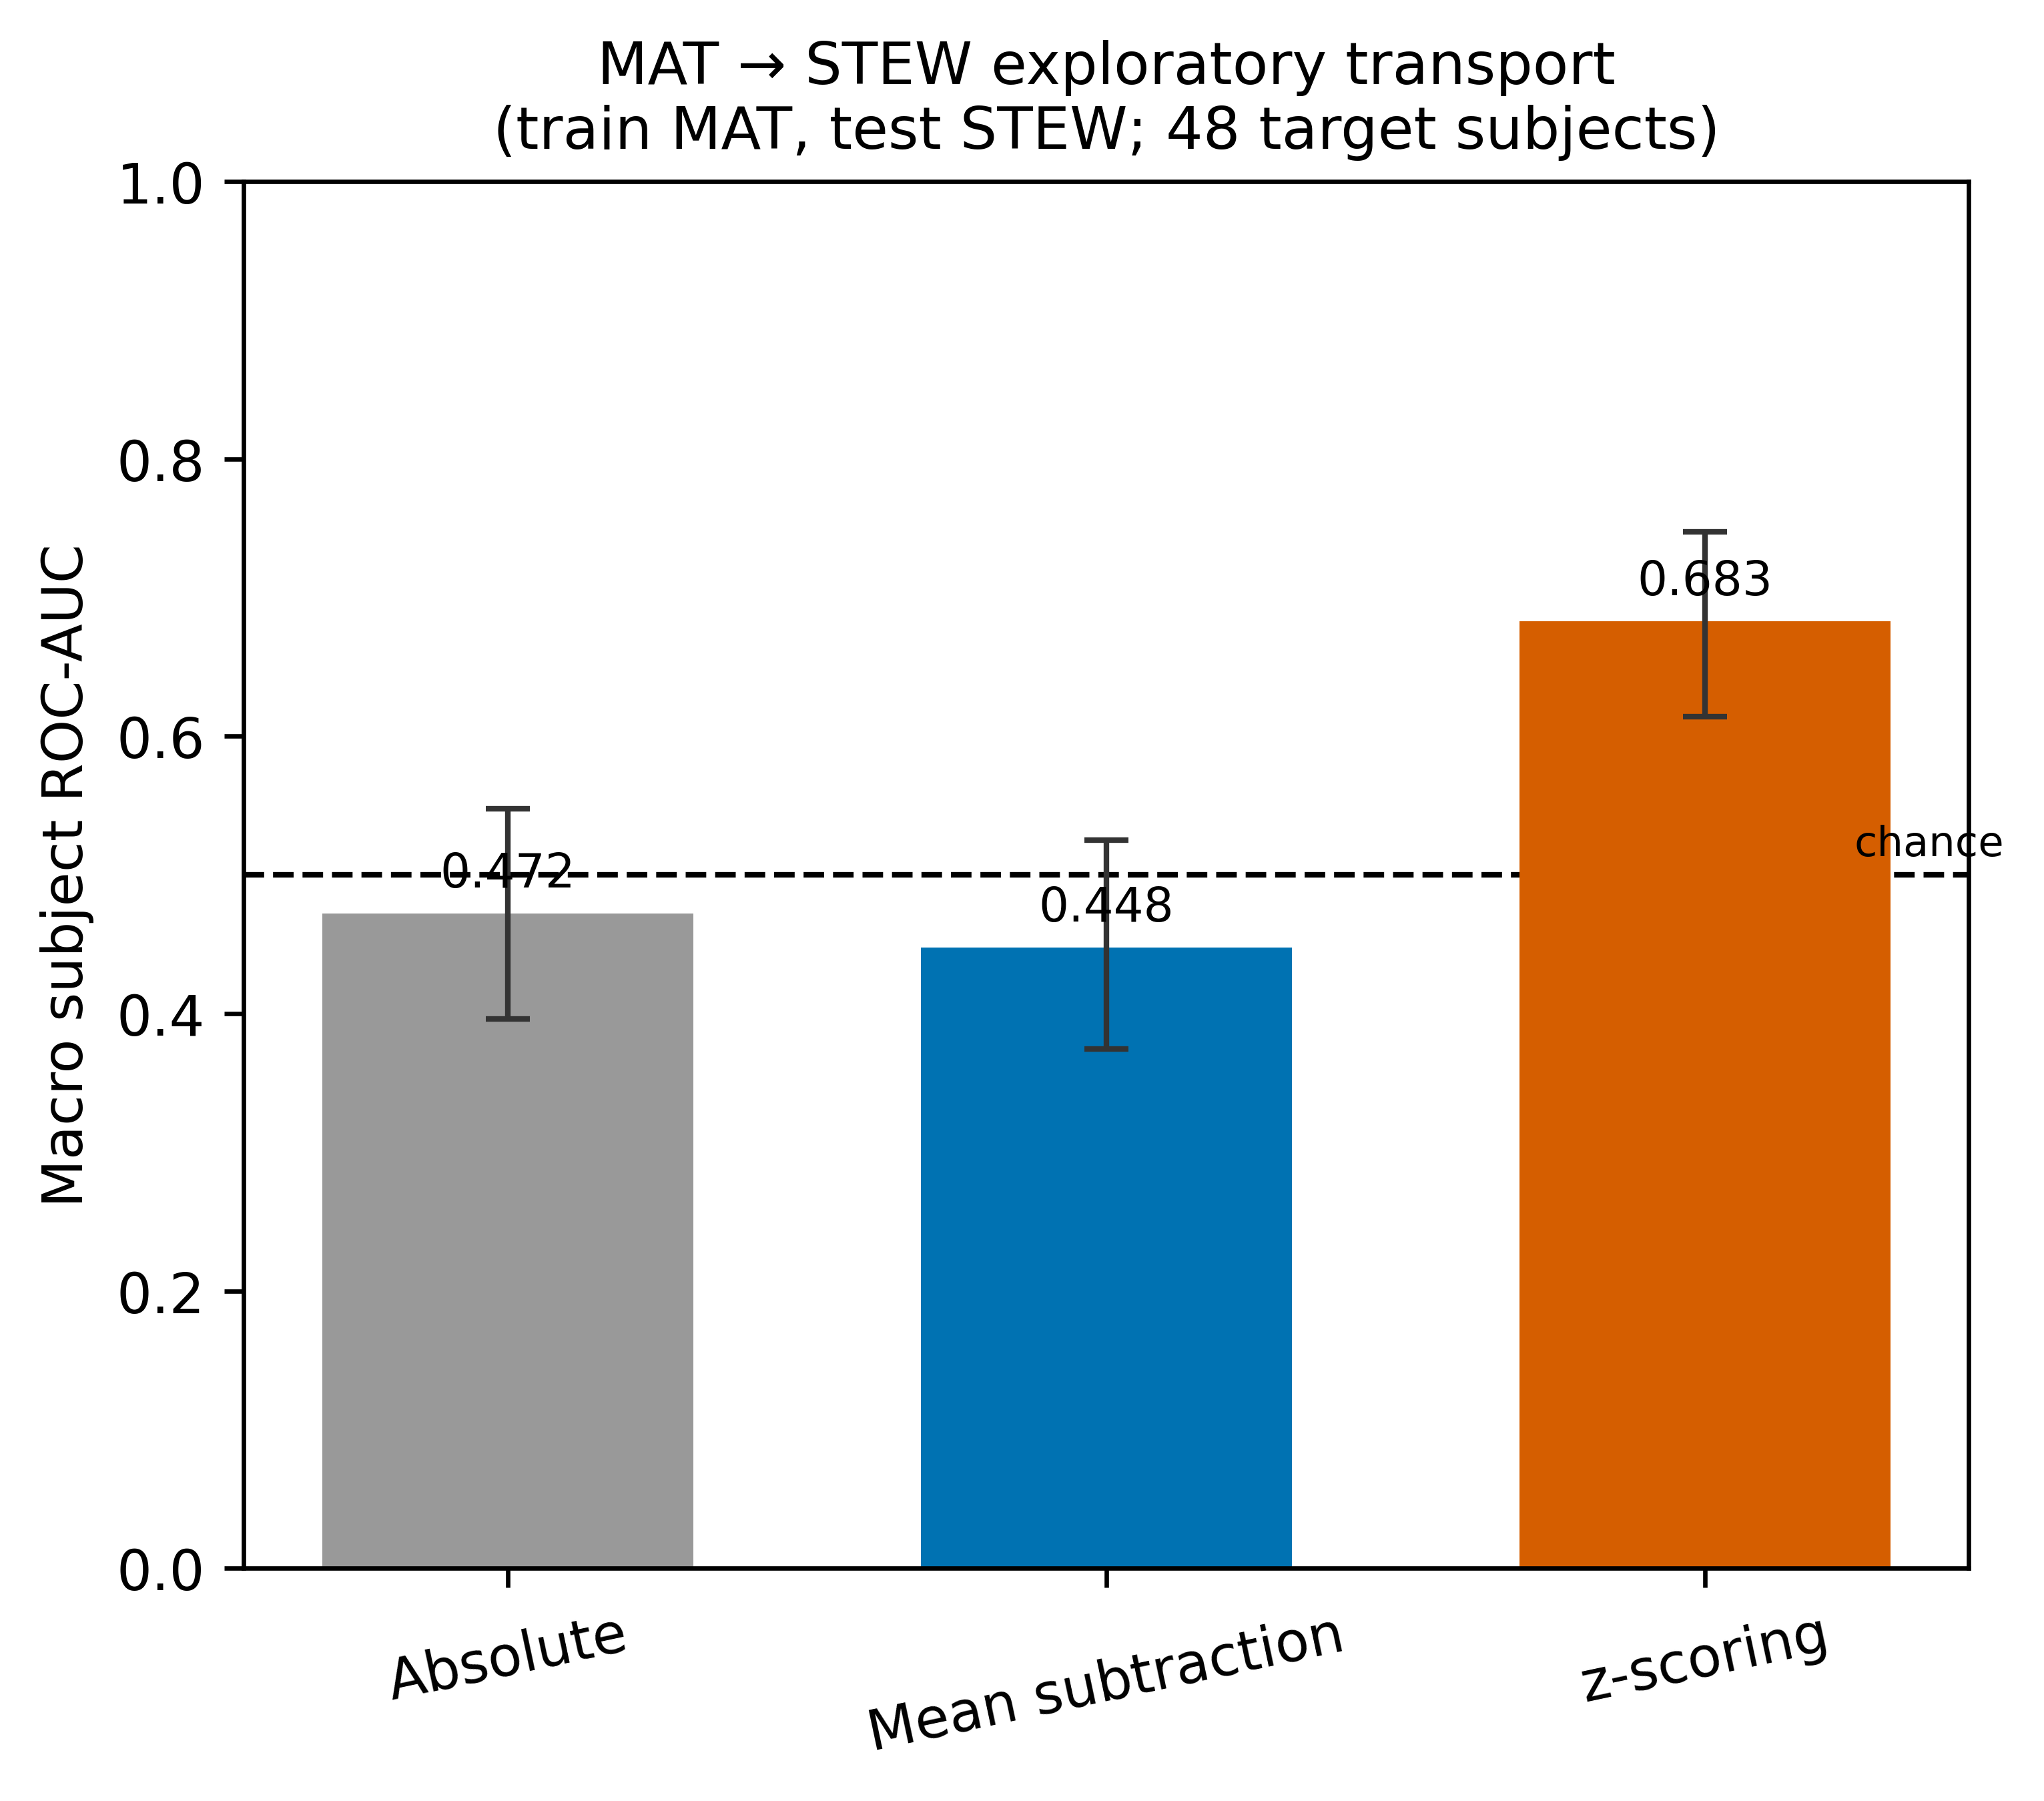
\includegraphics[width=0.6\linewidth]{../figures/figure_neg_mat_to_stew.png}
\caption{MAT$\rightarrow$STEW exploratory transport. The predeclared candidate
(mean subtraction) is below chance; only the post-hoc z-scoring diagnostic
exceeds chance. Error bars are subject-bootstrap $95\%$ CIs.}
\label{fig:transport}
\end{figure}

\begin{figure}[ht]
\centering
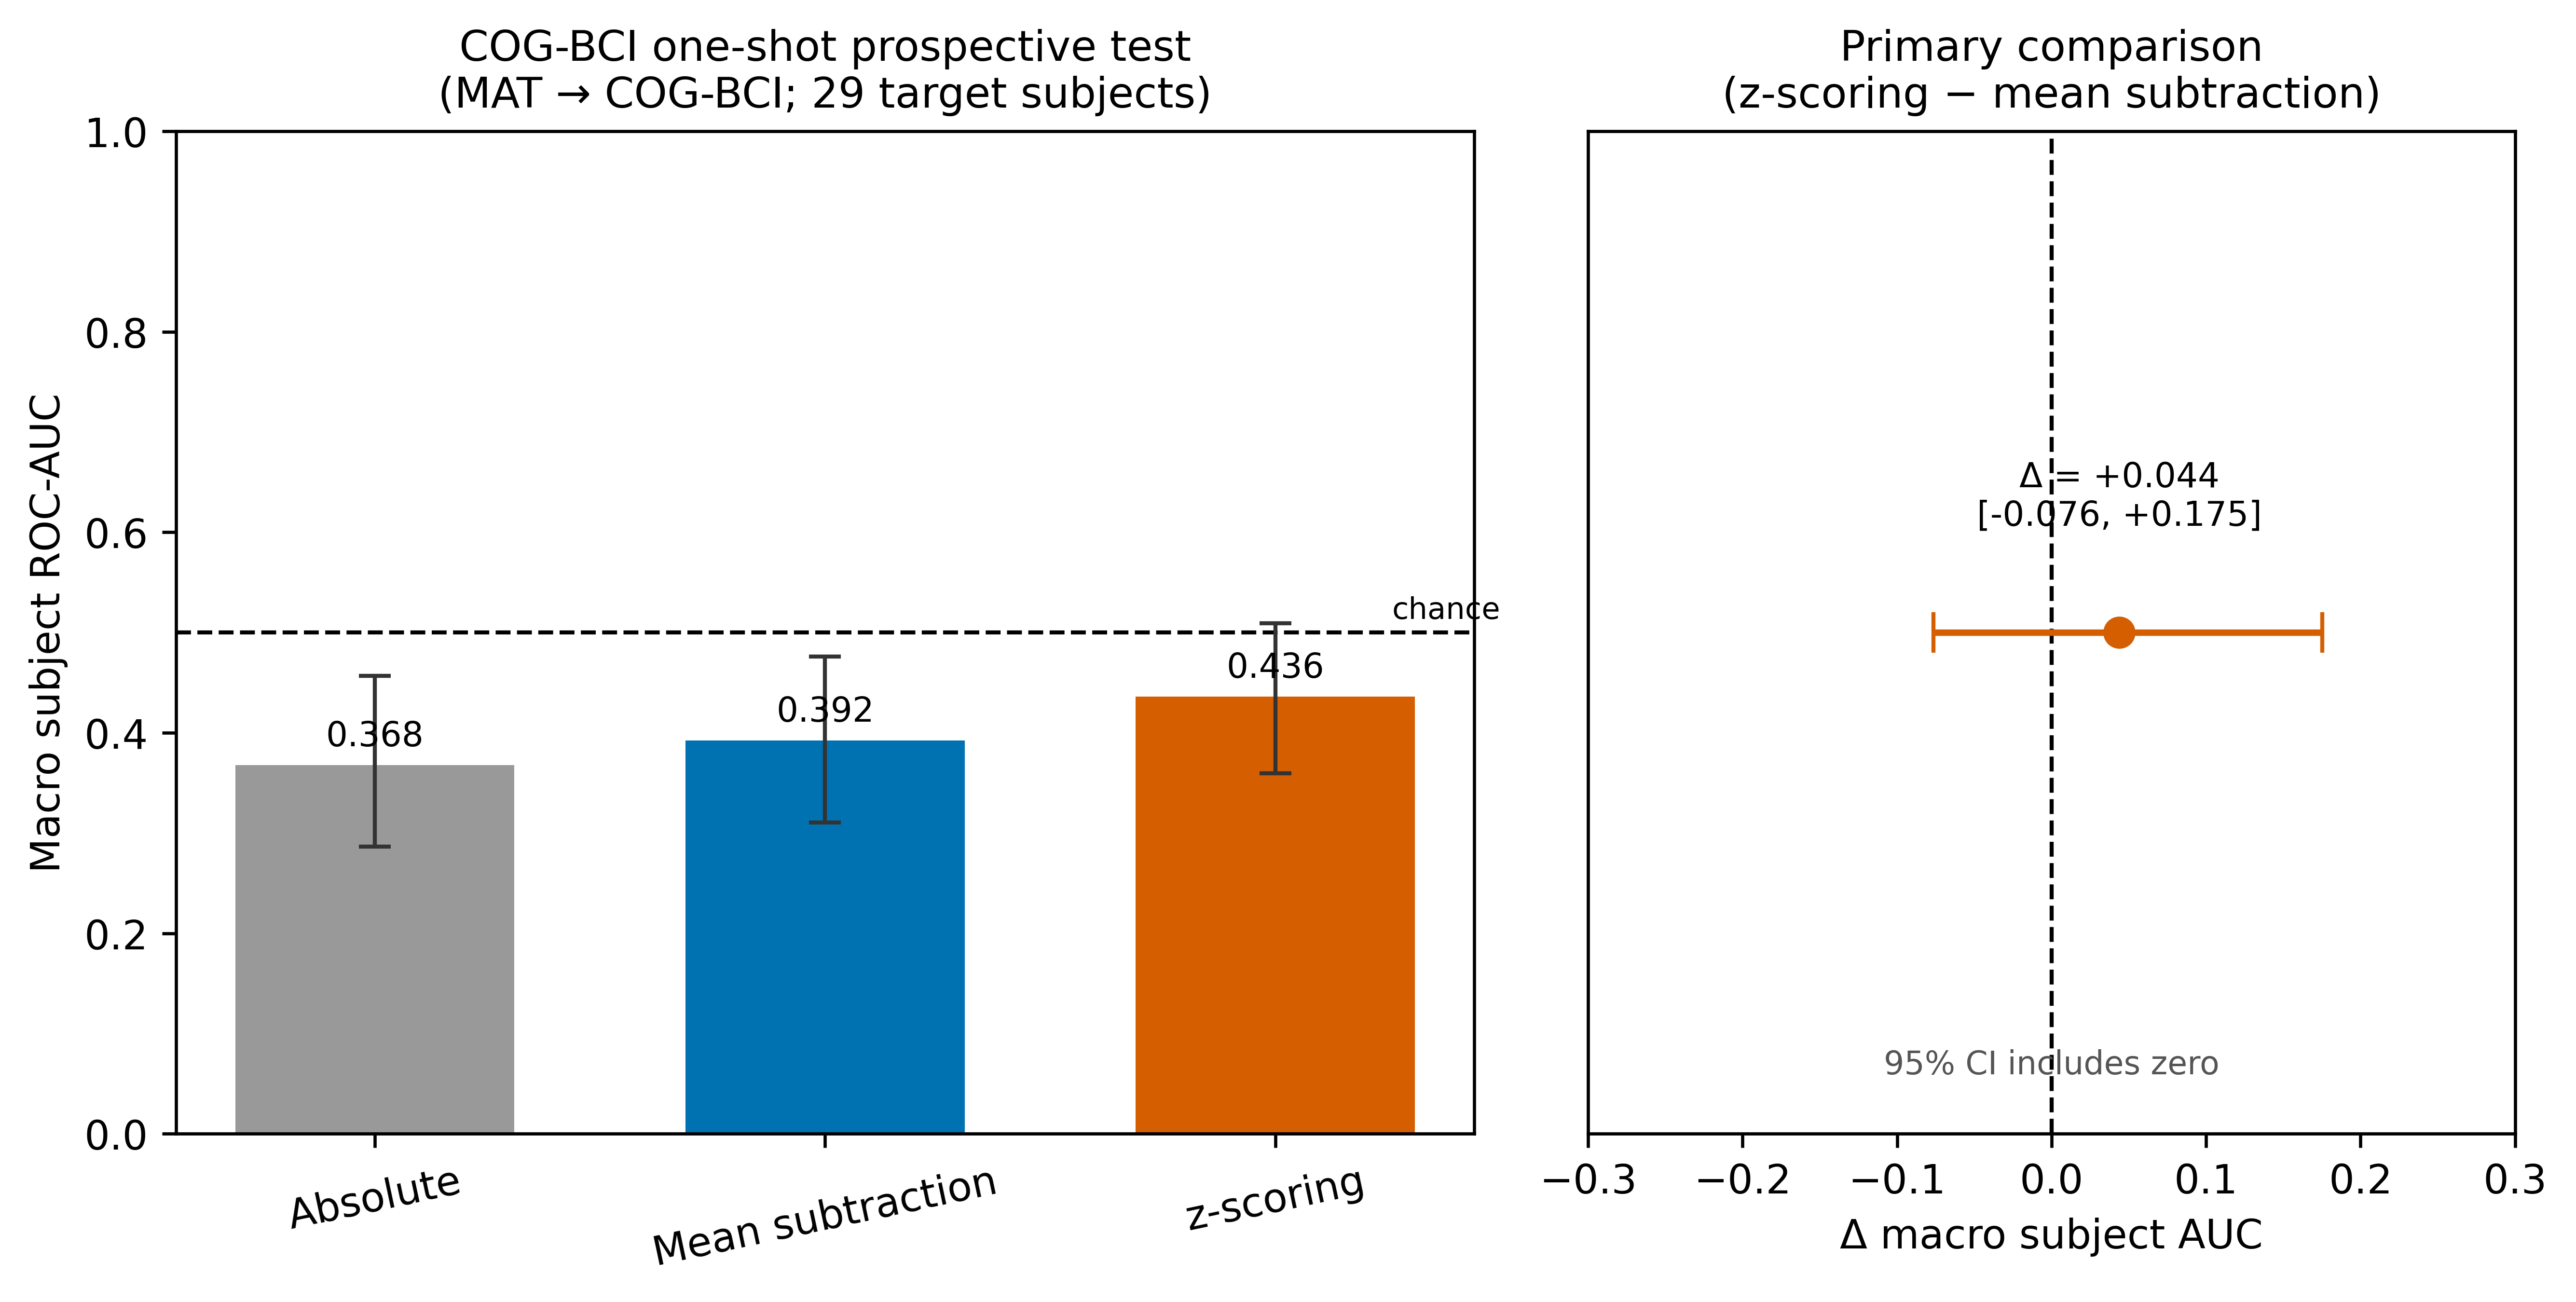
\includegraphics[width=0.95\linewidth]{../figures/figure_neg_cogbci_oneshot.png}
\caption{COG-BCI one-shot prospective test. Left: macro subject-level ROC-AUC by
calibration mode (all below chance). Right: the primary paired contrast
(z-scoring $-$ mean subtraction) with $95\%$ CI including zero. Error bars are
subject-bootstrap $95\%$ CIs; dashed lines mark chance (left) and zero (right).}
\label{fig:cogbci}
\end{figure}

\section{Discussion}

The principal finding is methodological: strong within-domain EEG workload
decoding did \textbf{not} imply transportability. Mean-subtraction calibration
decoded workload above chance within MAT (0.880) and within STEW (0.840), with
permutation $p \approx 0.005$ in each dataset, yet the predeclared
MAT$\rightarrow$STEW transport of that same calibrated pipeline fell below
chance (0.448). A post-hoc z-scoring observation that looked promising on STEW
(0.683) did not survive a single honest prospective test on untouched COG-BCI,
where every calibration mode transported below chance and the z-scoring
advantage over mean subtraction was statistically indistinguishable from zero.
High LOSO accuracy inside a dataset is thus not evidence of device/task
generalization.

We make no neural-mechanism claim. The features that drive within-dataset
decoding (band ratios, Hjorth parameters, spectral entropy) are not interpreted
physiologically, and no source-localization, anatomical-generator, or coupling
analysis was performed. Task, device, reference montage, amplitude units, and
cohort all differ across the three datasets; we treat these as plausible,
non-exclusive contributors to the transport failure, \textbf{not} as proven
causes, and the present analyses do not adjudicate among them. Below-chance
transport may reflect an anti-aligned decision geometry across domains, but we
do not interpret it mechanistically.

The contribution is the discipline of the test, not a positive result. We froze
the pipeline before the prospective evaluation, controlled leakage by fitting
only on the source dataset and calibrating from unlabeled baseline segments,
restricted transport to scale/offset-invariant features given undocumented STEW
units, harmonized the sampling representation transparently, and executed the
prospective test exactly once under checksum locks. Honest prospective
falsification of a post-hoc rescue is informative for reproducible BCI
methodology: it bounds what subject-baseline calibration can be expected to do
across heterogeneous domains.

\subsection{Limitations}

First, the cross-domain shift is large and confounded: device and task differ
simultaneously between MAT, STEW, and COG-BCI, so the two cannot be separated.
Second, there is a single prospective target (COG-BCI), tested once by design;
this maximizes inferential honesty but limits breadth. Third, the model and
feature family are fixed (one linear classifier; one feature set; eight
harmonized channels), so the result speaks to this pipeline, not to all possible
decoders. Fourth, STEW is an exploratory, non-comparable sensitivity dataset
with undocumented amplitude units, not a strict replication. Fifth, the analysis
was restricted to MATB-difficult versus eyes-open rest; N-back, other MATB
levels, eyes-closed rest, and COG-BCI sessions S2/S3 were prespecified out of
scope and contribute no results. Sixth, no permutation test was computed for the
COG-BCI run (outside the frozen script's scope); it is not needed because the
primary endpoint was already below chance. Finally, the study supports no
clinical, deployment, diagnostic, real-time, mechanistic, anatomical, or causal
claim, and reports no estimate of publication likelihood.

\section{Conclusion}

Across three provenance-distinct EEG datasets, baseline-relative processing
supported \textbf{within-domain} workload decoding (mean-subtraction macro
subject AUC 0.880 within MAT and 0.840 within STEW, each $p \approx 0.005$), but
neither mean subtraction nor the prospectively tested z-scoring supported
\textbf{cross-domain} transport of the MAT-trained decoder. The predeclared
MAT$\rightarrow$STEW mean-subtraction transport failed below chance (0.448), and
the frozen one-shot COG-BCI prospective test of the post-hoc z-scoring
hypothesis also failed below chance (0.436; primary $\Delta$AUC CI includes
zero). Under the specific task and device shifts tested here, strong
within-dataset decoding did not establish a transportable workload decoder. We
report this as a rigorous negative transport/reproducibility result.

\section{Data and Code Availability}

The original datasets are available from PhysioNet EEGMAT
\cite{physionet_eegmat}, IEEE DataPort STEW \cite{stew_dataset}, and the COG-BCI
database \cite{hinss2023}. Raw EEG signals are not redistributed here. The
analysis code, frozen configurations, checksum manifests, and committed
result-summary files are stored in the project repository; the decisive
summaries are \texttt{MAT\_MEAN\_SUBTRACTION\_SUBJECT\_LEVEL\_RESULTS.md},
\texttt{MAT\_MACRO\_SUBJECT\_NULL\_RESULTS.md},
\texttt{STEW\_EXPLORATORY\_SENSITIVITY\_RESULTS.md},
\texttt{MAT\_TO\_STEW\_EXPLORATORY\_TRANSFER\_RESULTS.md},
\texttt{COG\_BCI\_ONE\_SHOT\_PROSPECTIVE\_RESULTS.md}, and the artifacts under
\texttt{results/cog\_bci\_one\_shot/} (including \texttt{RUN\_MARKER.json} and
\texttt{config\_and\_script\_checksums.json}).

\section{Ethics Statement}

This work is a secondary analysis of publicly available, de-identified EEG
datasets. No new human-subject data were collected. The original datasets were
collected under their respective ethics approvals and consent procedures. The
present work is intended for computational and methodological research, not
clinical diagnosis or individual assessment.

\section{Author Contributions}

Arush Ravipati and Abhijay Gangarapu contributed equally to the conception,
analysis, interpretation, and manuscript preparation for this study.

\section{Conflict of Interest}

The authors declare no commercial or financial relationships that could be
construed as a potential conflict of interest.

\section{Acknowledgments}

The authors thank the creators of the PhysioNet EEGMAT, IEEE DataPort STEW, and
COG-BCI datasets for making their data publicly available.

\begin{thebibliography}{99}
\bibitem{klimesch1999} Klimesch W. EEG alpha and theta oscillations reflect cognitive and memory performance: a review and analysis. Brain Research Reviews. 1999;29(2-3):169-195.
\bibitem{gevins1997} Gevins A, Smith ME, McEvoy L, Yu D. High-resolution EEG mapping of cortical activation related to working memory: effects of task difficulty, type of processing, and practice. Cerebral Cortex. 1997;7(4):374-385.
\bibitem{sridhar2022} Sridhar S, Manian V, Rao RPN. Theta and alpha ratios as objective correlates of cognitive workload: a cross-task replication study. Journal of Neural Engineering. 2022;19(4):046033.
\bibitem{zyma2019} Zyma I, Tukaev S, Seleznov I, Kiyono K, Popov A, Chernykh M, Shpenkov O. Electroencephalograms during Mental Arithmetic Task Performance. Data. 2019;4(1):14.
\bibitem{lotte2018} Lotte F, Bougrain L, Cichocki A, Clerc M, Congedo M, Rakotomamonjy A, Yger F. A review of classification algorithms for EEG-based brain-computer interfaces: a 10 year update. Journal of Neural Engineering. 2018;15(3):031005.
\bibitem{physionet_eegmat} Zyma I, Tukaev S, Seleznov I, Kiyono K, Popov A, Chernykh M, Shpenkov O. EEG During Mental Arithmetic Tasks [Dataset]. PhysioNet. 2019. https://doi.org/10.13026/C2JQ1P.
\bibitem{stew_dataset} Lim WL, Sourina O, Wang LP. STEW: Simultaneous task EEG workload data set. IEEE Transactions on Neural Systems and Rehabilitation Engineering. 2018;26(11):2106-2114.
\bibitem{openneuro_ds007262} Barras M, Booth L. Cognitive Workload 8-level Arithmetic Task. OpenNeuro DS007262. 2026. https://doi.org/10.18112/openneuro.ds007262.v1.0.6.
\bibitem{mne} Gramfort A, Luessi M, Larson E, Engemann DA, Strohmeier D, Brodbeck C, Goj R, Jas M, Brooks T, Parkkonen L, Hamalainen M. MEG and EEG data analysis with MNE-Python. Frontiers in Neuroscience. 2013;7:267.
\bibitem{jayaram2016} Jayaram V, Alamgir M, Altun Y, Scholkopf B, Grosse-Wentrup M. Transfer learning in brain-computer interfaces. IEEE Computational Intelligence Magazine. 2016;11(1):20-31.
\bibitem{hakimi2023} Hakimi N, Jodeiri A, Setarehdan SK. Mental arithmetic task classification using convolutional neural networks on EEG signals. Biomedical Signal Processing and Control. 2023;79:104156.
\bibitem{roy2016} Roy RN, Charbonnier S, Campagne A, Bonnet S. Efficient mental workload estimation using task-independent EEG features. Journal of Neural Engineering. 2016;13(2):026019.
\bibitem{jebelli2019} Jebelli H, Hwang S, Lee S. EEG-based workers' mental workload classification using deep learning. Automation in Construction. 2019;106:102876.
\bibitem{nguyen2025} Nguyen PK, Huynh QL. A machine learning approach in EEG-based assessment of cognitive load by mental arithmetic tasks. Journal of Physics: Conference Series. 2025;2949:012004.
\bibitem{borghini2014} Borghini G, Astolfi L, Vecchiato G, Mattia D, Babiloni F. Measuring neurophysiological signals in aircraft pilots and car drivers for the assessment of mental workload, fatigue and drowsiness. Neuroscience \& Biobehavioral Reviews. 2014;44:58-75.
\bibitem{cavanagh2014} Cavanagh JF, Shackman AJ. Frontal midline theta reflects anxiety and cognitive control: a meta-analytic review. Journal of Physiology-Paris. 2014;108(4-6):251-258.
\bibitem{sweller1988} Sweller J. Cognitive load during problem solving: effects on learning. Cognitive Science. 1988;12(2):257-285.
\bibitem{hart1988} Hart SG, Staveland LE. Development of NASA-TLX (Task Load Index): results of empirical and theoretical research. Advances in Psychology. 1988;52:139-183.
\bibitem{gramfort2013} Gramfort A, Luessi M, Larson E, Engemann DA, Strohmeier D, Brodbeck C, Goj R, Jas M, Brooks T, Parkkonen L, Hamalainen M. MEG and EEG data analysis with MNE-Python. Frontiers in Neuroscience. 2013;7:267.
\bibitem{sklearn} Pedregosa F, Varoquaux G, Gramfort A, Michel V, Thirion B, Grisel O, et al. Scikit-learn: Machine learning in Python. Journal of Machine Learning Research. 2011;12:2825-2830.
\bibitem{zander2011} Zander TO, Kothe C. Towards passive brain-computer interfaces: applying brain-computer interface technology to human-machine systems in general. Journal of Neural Engineering. 2011;8(2):025005.
\bibitem{vidaurre2011} Vidaurre C, Sannelli C, Muller KR, Blankertz B. Co-adaptive calibration to improve BCI performance. NeuroImage. 2011;55(4):1443-1456.
\bibitem{congedo2017} Congedo M, Barachant A, Bhatia A. Riemannian geometry for EEG-based brain-computer interfaces: a primer and a review. Brain-Computer Interfaces. 2017;4(3):155-174.
\bibitem{baldwin2013} Baldwin CL, Penaranda BN. Adaptive training using an artificial neural network and EEG metrics for within- and cross-task workload classification. NeuroImage. 2013;59(1):48-56.
\bibitem{goldberger2000} Goldberger AL, Amaral LAN, Glass L, Hausdorff JM, Ivanov PC, Mark RG, et al. PhysioBank, PhysioToolkit, and PhysioNet: Components of a new research resource for complex physiologic signals. Circulation. 2000;101(23):e215-e220.
\bibitem{wong2011} Wong B. Points of view: Color blindness. Nature Methods. 2011;8(6):441.
\bibitem{zanini2018} Zanini P, Congedo M, Jutten C, Said S, Berthoumieu Y. Transfer learning: a Riemannian geometry framework with applications to brain-computer interfaces. IEEE Transactions on Biomedical Engineering. 2018;65(5):1107-1116.
\end{thebibliography}


\end{document}
